\documentclass[norsk,a4paper,12pt]{article}
\usepackage[utf8]{inputenc}
\usepackage{graphicx} %for å inkludere grafikk
\usepackage{verbatim} %for å inkludere filer med tegn LaTeX ikke liker
\usepackage{tabularx}
\usepackage{booktabs}
\usepackage{amsmath}
\usepackage{float}
\usepackage{color}
\usepackage{listings}
\usepackage{hyperref}
\lstset{language=c++}
\lstset{basicstyle=\small}
\lstset{backgroundcolor=\color{white}}
\lstset{frame=single}
\lstset{stringstyle=\ttfamily}
\lstset{keywordstyle=\color{red}\bfseries}
\lstset{commentstyle=\itshape\color{blue}}
\lstset{showspaces=false}
\lstset{showstringspaces=false}
\lstset{showtabs=false}
\lstset{breaklines}
\lstset{postbreak=\raisebox{0ex}[0ex][0ex]{\ensuremath{\color{red}\hookrightarrow\space}}}
\usepackage{titlesec}

\setcounter{secnumdepth}{4}

\titleformat{\paragraph}
{\normalfont\normalsize\bfseries}{\theparagraph}{1em}{}
\titlespacing*{\paragraph}
{0pt}{3.25ex plus 1ex minus .2ex}{1.5ex plus .2ex}


\title{FYS3150 - Computational Physics\\\vspace{2mm} \Large{Project 3}}
\author{\large Richard Andr\'e Fauli\\ Dorthea Gjestvang\\ Even Marius Nordhagen}
\date{\today}
\begin{document}

\maketitle
\begin{abstract}
This project aims to use ODE solvers on orbiting planets. For a simple two-body system we compare the Euler-Cromer and the Velocity Verlet methods. We then use Velocity Verlet to model Earth-Jupiter-Sun systems, the solar system and the perihelion precession of Mercury.

We found that Velocity Verlet had a higher numerical precision than Euler-Cromer but was about $50\%$ more time consuming. For different choices of Jupiter-masses, the Earth-Jupiter-Sun system behaved as expected. Our implementation of the solar system was stable for at least a hundred years with time step $dt=10^{-3}$. However the perihelion precession of Mercury was found to be several time larger than expected.\end{abstract}
\begin{itemize}
\item Github repository containing programs and results are in: \url{https://github.com/richaraf/Comphys_projects/tree/master/Project_3}
\end{itemize}
\section{Introduction}
The solar system is a complex system consisting, among other things, of a star, eight planets and several moons. Newton's law of gravity gives that the force acting between each pairs of bodies in the system is described by equation \ref{eq:GravityForce}

\begin{equation}
    F_G = \frac{G m_1 m_2}{|\vec{r}|^3}\vec{r}.
    \label{eq:GravityForce}
\end{equation}

If we want to obtain the motion of the planets using equation \ref{eq:GravityForce} and Newtons laws of motion,  we get a set of coupled differential equations. Solving these equations has been a goal for physicists for several centuries, but before the age of computers, this was tiresome.
\par 
\vspace{2mm}
In this project, our goal is to simulate the solar system as accurately as possible. We start by implementing a simplified two body system, consisting of the Sun and the Earth, by rewriting equation \ref{eq:GravityForce} as a set of coupled differential equations for the positions and velocity of the two bodies. We assume circular orbit and neglect the motion of the Sun. The theory behind the rewriting of these equations is presented in section 2.1.  We check the stability of the system using the ODE-solvers EulerCromer and VelocityVerlet, presented in section 3.1,  for different timesteps $dt$, and study the conservation of energy and angular momentum. When this simulation runs as required, we add Jupiter, and solve the motion for the three body system, again looking at the stability of the system. 
\par
\vspace{2mm}
Thereafter we implement a more realistic model for the entire solar system using the planet's actual elliptical orbits including the movement of the Sun around the center of mass. The theory is presented in section 2.4. We then use our model to observe the difference a relativistic Newtonian gravity force makes on the perihelion precession of Mercury. Finally, in section 4 and 5 we present and discuss our results.
\section{Theory}
In this project we are simulating the planet orbits of the solar system by using Newton's laws of motion. Newton's second law states that the total force acting on an object with mass $m$ is given by
\begin{equation}
\Sigma\vec{F}=m\vec{a}
\label{eq:N2L}
\end{equation}
where $\Sigma \vec{F}$ is the sum of the forces acting on the object and $\vec{a}$ is the acceleration. In our case we are going to use this reversed, with finding the acceleration when we already know the force on an object and the mass of the object. Since we are going to deal with long distances, heavy objects and high velocities, we will use astronomical units such as average distance between Earth and the sun, AU, (1AU $\approx1.5\cdot10^{11}$m), Solar mass $M_\odot$ ($1M_{\odot}\approx2\cdot10^{30}$ kg) and velocity in AU/$yr$, while the time has unit years, $yr$. The constants are taken from the Project instructions \cite {Project_text}. In space we do not have any friction, so all forces come from gravitation between planets, stars and other objects. Newton's universal law of gravitation between two objects is given by equation (\ref{eq:GravityForce})
where $G$ is the gravitational constant, $m_1$ and $m_2$ are the masses of the objects, $\vec{r}$ is a vector representing the distance between them. Since we are using astronomical units, this gives the value $G = 4\pi^2 M_{\odot} ^{-1} AU^3 yr^{-2}$ \cite{Project_text} for the gravitational constant.  The absolute gravitational force between two objects is therefore
\begin{equation}
F_G=-G\frac{m_1\cdot m_2}{r^2}.
\label{eq:absGravitationalForce}
\end{equation}
The gravitational force is a conservative force, which means it conservs mechanical energy\cite{Concervative_Force}. The total mechanical energy, the sum of the potential and the kinetic energy, should therefore be conserved in our model.

We are also going to deal with the Barycenter (the center of mass for a system with two or more objects), which is defined as the point where we have equal masses in all directions. For a solar system, this can mathematically be written as
\begin{equation}
\vec{R}=\sum_{i=1}^N \frac{m_i}{M}\vec{r}
\end{equation}
where $N$ is the number of objects, $m_i$ is the mass of object $i$, $\vec{r}_i$ is the position of the mass center of object $i$ and $M$ is the total mass of the system \cite{Barycenter}.\par\vspace{5mm}

Another physical concept which we are going to use to check the stability of the solar system is the angular momentum. Angular momentum is defined as the cross product between the position vector $\vec{r}$ and the momentum vector $\vec{p}$:
\begin{equation}
L=\vec{r}\times\vec{p}.
\end{equation}
where we assume that the centre of rotation is set to the origin. The solar system is a global system (not affected by other systems), and the conservation laws will always hold. This means that we do not have any external torque, so the angular momentum must be conserved. 
\subsection{Two-body System}
Initially we are studying the two-body problem with the Sun fixed to origin and with Earth orbiting the Sun. This is not fully correct, since the size of the force on the Sun is the same as the size of the force on Earth (Newton's third law). Anyway this is still a good approximation because the mass of Sun is much larger than that of Earth, such that the movement of the Sun becomes negligible. The Earth's orbit around the Sun is co-planar (two-dimensional), so we are decomposing the force in two directions, and from Equation (\ref{eq:N2L}) we obtain
\begin{equation}
a_x=\frac{d^2x}{dt^2}=\frac{F_{G,x}}{M_{Earth}}
\end{equation}
and
\begin{equation}
a_y=\frac{d^2y}{dt^2}=\frac{F_{G,y}}{M_{Earth}}.
\end{equation}
Where $F_{G,x}$ and $F_{G,y}$ are the forces acting on Earth in respectively x-direction and y-direction. By inserting Equation (\ref{eq:GravityForce}) into these equations, we can calculate the total acceleration of Earth in the $x$ and $y$ directions:
\begin{equation}
\frac{d^2x}{dt^2}=-G\frac{M_\odot}{r^3}x
\end{equation}
\begin{equation}
\frac{d^2y}{dt^2}=-G\frac{M_\odot}{r^3}y
\end{equation}
We can use the acceleration in compliance with an integration method and find the position and velocity after a time $dt$ using the discrete version of Newton's second law. Examples of such integration methods are the Euler-Cromer method and the Velocity Verlet method. By doing this $N$ times, we can compute the motion for $N\cdot dt$ years. 

In the two-body case the velocity of Earth is set to the analytical velocity which gives a circular orbit. 
 
\subsection{Gravitational theory}
\subsubsection{Circular Orbit}
In the Solar system the orbits of the planets are elliptical, with the Sun in one of the foci \cite{kepler}. In the two-body- and three-body parts of this system, we assume circular orbits for the planets we study. To get circular orbits, we have to assume that $M_{\odot} >> M_{planet}$, and that the Sun stands still in the center of mass of the system. \par
\vspace{3mm}

For setting the initial velocity of the planets, we need the orbital velocity of a circular orbit. The centripetal force is the force that makes an object follow a curved path, and its magnitude is given by equation \ref{eq:CentripetalForce}, where $m$ is the mass of the object, $v$ is the tangential velocity and $r$ is the radius of the circular path. 

\begin{equation}
     F_c = m \frac{v^2}{r}
     \label{eq:CentripetalForce}
\end{equation}

For a circular orbit, the centripetal force $F_c$ must be equal to the gravitational force, given by equation \ref{eq:GravityForce}, where we use $m = m_1$ and $M =m_2$. We can now calculate the orbital velocity $v_{orb}$ of a circular orbit with radius r:

\begin{equation}
    F_c = F_G \quad \quad m \frac{v_{orb}^2}{r} = \frac{GmM}{r^2} \quad \Rightarrow \quad v_{orb} = \sqrt{\frac{GM}{r}}
    \label{eq:OrbitalVelocity}
\end{equation}

The average distance between the Earth and the Sun is $1 AU$, so the orbital velocity of the Earth in a circular orbit is

\begin{equation}
v_{orb} = \sqrt{\frac{GM}{r}} = \sqrt{\frac{ 4\pi^2 M_{\odot} ^{-1} AU^3 yr^{-2} M_{\odot}}{1 AU}} = 2\pi AU/yr 
\label{eq:AnalyticVel}
\end{equation}

We also need the orbital velocity of Jupiter in a circular orbit. By using equation \ref{eq:OrbitalVelocity} and the average distance between the Sun and Jupiter, $r = 5.20 AU$ \cite{Project_text}, we find that the velocity of Jupiter in our circular orbit approximation is $\approx 2.755 AU/yr$.

\subsubsection{Escape velocity}
A two body system consists of two objects, object 1 with mass $m_1$ and object 2 with mass $m_2$. The kinetic energy of object 1 is given by equation \ref{eq:kineticE}, where $v$ is object 1's velocity with respect to the center of mass. The potential energy of object 1 in the gravitational field between the two objects, is given by equation \ref{eq:potE}, where G is the gravitational constant and $|\vec{r}|$ is the distance between the two objects. 

\begin{equation}
    E_k = \frac{1}{2} m_1 v^2
    \label{eq:kineticE}
\end{equation}

\begin{equation}
    E_p = - \frac{G m_1 m_2}{|\vec{r}|}
    \label{eq:potE}
\end{equation}
\par 
\vspace{3mm}

Per definition, the escape velocity of an object is at the point when the object's total energy $E_k + E_p$ is equal to zero \cite{kepler}. This gives us a way to compute the escape velocity, $v_{esc}$:

\begin{equation*}
    E_k + E_p = 0 \qquad \rightarrow \qquad \frac{1}{2} m v_{esc}^2 - \frac{G m M}{|\vec{r}|} = 0
\end{equation*}

\begin{equation}
     v_{esc}^2 = \frac{2 G M}{|\vec{r}|} \quad \Rightarrow \quad v_{esc} = \sqrt{\frac{2 G M}{|\vec{r}|}}
     \label{esc_v}
\end{equation}

For an object in a distance $|\vec{r}| = 1AU$ from the Sun (as is the case for the Earth), the escape velocity $v_{esc}$ is 

\begin{equation*}
    v_{esc} = \sqrt{\frac{2 G M}{|\vec{r}|}} = \sqrt{\frac{2 * 4\pi^2 M_{\odot} ^{-1} AU^3 yr^{-2} * M_{\odot}}{1 AU}} = \sqrt{8}\pi AU/yr \approx 8.886 AU/yr
\end{equation*}

If we want to check numerically whether a planet is trappet in a gravitational field or escapes, we can implement a test that checks if the total energy of the planet $E = E_k + E_p$ is smaller or bigger than a given tolerance. If the total energy is bigger that the tolerance, the planet is not bound in the gravitational field, and will escape.

\subsection{Three-Body System}
Furthermore we have a three-body system where the most massive planet in the solar system, Jupiter, is set to a circular orbit around the Sun while Earth is still orbiting the sun by a distance 1AU with the sun kept fixed to the origin. For the two-body system we found an analytical solution for the motion, but in this case this is hard, if not impossible, because of the interaction between the planets. Nevertheless we can solve it numerically by using the same equations as for the two-body system. For each "time-step" $dt$ we now need to update the position and velocity for both planets where we also compute the interaction forces between them. 

\subsection{Solar System (Many-body System)}
The implementation of the many-body system is very similar to the three-body system, the main difference is that we will have many more forces. Every time we add a new object, the new object will have forces acting on all other objects, so we will have $N-1$ new forces where $N$ is the total number of objects. The total number of forces acting on a many-body system is therefore given by
\begin{equation}
P(N)=\sum_{i=1}^N(i-1)=\sum_{i=0}^{N-1}i=\frac{N(N-1)}{2}.
\end{equation}
where the last transition can be found in a collection of mathematical formulae.  We will also look at the real case when all the objects in the solar system are orbiting a barycentre (center of mass). When we implement the model, we do not need equations for all the forces, but we need one equation for the position and velocity in each direction for all the objects. We will therefore need $2\cdot2\cdot8=32$ equations to implement a model for our solar system with 8 planets and the sun in two dimensions. For this we need the masses, initial positions in relation to the barycentre and initial velocities for all the planets and the sun. The masses and distances to Sun are found in Table (\ref{tab:Masses}).
\begin{table}[H]
\centering
\caption{Masses and distances to sun for all planets in the solar system, given in respectively $M_\odot$ and AU.}
\label{tab:Masses} 
\begin{tabularx}{\textwidth}{lXcccXr}
\toprule
Planet  &   & Mass [$M_\odot$] &    & Distances from Sun [AU] \\
\midrule
Mercury 	&	& 1.66051E-07  &    & 0.39    \\
Venus   &   & 2.44827E-06  &    & 0.72    \\
Earth   &   & 3.00329E-06  &    & 1.00    \\
Mars    &   & 3.22774E-05  &    & 1.52    \\
Jupiter &   & 9.54533E-04  &    & 5.20    \\
Saturn 	&	& 2.85797E-04  &    & 9.54    \\
Uranus 	&	& 4.36552E-05  &    & 19.19   \\
Neptun  &	& 5.15000E-05  &    & 30.06   \\
\bottomrule
\end{tabularx}
\end{table}
The masses and distances in Table (\ref{tab:Masses}) are taken from the Project instructions \cite{Project_text}, and where we have reduced the number of decimals to 5, although we include 10 decimals in the program. The initial velocities and positions are found in Table ({\ref{tab:Positions}).
\begin{table}[H]
\centering
\caption{Initial positions relative to a centre of mass and velocities for all the planets in the solar system and the sun, given in respectively AU and AU/yr. These are actual data for October 12th 2016, downloaded from NASA.}
\label{tab:Positions}
\begin{tabularx}{\textwidth}{lrrrrr}
\toprule
\multicolumn{3}{r}{Positions [AU]} & \multicolumn{3}{r}{Velocities [AU/yr]} \\
\cline{2-3}
\cline{5-6}
Planet           & x & y &  & x & y \\
\midrule
Sun          & 3.57153E-03  & 3.38904E-03  & & -1.97008E-06 & 6.84622E-06  \\
Mercury      & -3.13025E-01 & 1.56078E-01  & & -1.80109E-02 & -2.41438E-02 \\
Venus        & 1.42294E-01  & -7.10557E-01 & & 1.97176E-02  & 3.79469E-03  \\
Earth        & 9.47918E-01  & 3.26107E-01  & & -5.84936E-03 & 1.62170E-02  \\
Mars         & 1.13700E+00  & -7.88667E-01 & & 8.54547E-03  & 1.26763E-02  \\
Jupiter      & -5.43013E+00 & -4.32084E-01 & & 5.12061E-04  & -7.16556E-03 \\
Saturn       & -2.28243E+00 & -9.77097E+00 & & 5.12605E-03  & -1.28636E-03 \\
Uranus 		 & 1.84678E+01  & 7.55105E+00  & & -1.51730E-03 & 3.45720E-03  \\
Neptun 		 & 2.82579E+01  & -9.93123E+00 & & 1.02007E-03  & 2.97988E-03  \\
\bottomrule
\end{tabularx}
\end{table}
NB: The data from NASA was given in three dimensions (x, y, z) but since we are studying the solar system in two dimensions (x, y), we have only included the data in x- and y-direction. This can introduce some errors, for example the velocity of the Earth changes slightly when we ignore the $z$ direction. \par\vspace{3mm}

\subsection{Mercury-Sun system}
Mercury's orbit around the sun has an observed perihelion precession of 43 arc seconds per century. To study this effect we make a relativistic correction to equation (\ref{eq:GravityForce}) meaning that the force acting on Mercury from the Sun becomes
\begin{equation}
F_G=-G\frac{m_1\cdot m_2}{r^2} \left[1 + \frac{3l^2}{r^2c^2}\right], 
\label{eq:GravitationalForceRelativistic}
\end{equation}
where $l$ is the magnitude of Mercury's orbital angular momentum per unit mass and $c$ is the speed of light in vacuum. 

If we give Mercury initial position on the $x$-axis such that $y=0$, we can find the perihelion angle $\theta_p$
\begin{equation}
\text{tan }\theta_p = \frac{y_p}{x_p},
\label{eq:perihelionangle}
\end{equation}
where $x_p$ and $y_p$ give the position of Mercury at perihelion.
\section{Method}
\subsection{Ordinary differential equation solvers}
In this project we use two different ODE solvers, the Euler-Cromer method and the velocity Verlet method. Both are derived using Taylor expansions to respectfully second and third order. For sufficiently small timesteps $dt$, both these methods should conserve energy for conservative forces such as the gravitational force. In both methods we are looking at a system with position $x_i$ and velocity $v_i$ at step number $i$, where $x_0$ and $v_0$ are known initial conditions.
\subsubsection{Euler-Cromer}
To find an algorithm for Euler-Cromer we first estimate the velocity at step $i+1$, $v_{i+1}$, by doing a second order Taylor expansion of the velocity 
\begin{equation}
v_{i+1} = v_i + dtv_i^{(1)} + {\cal O}(dt^2). 
\label{eq:EulCrov}
\end{equation}
We can then use $v_{i+1}$ to find the position at step $i+1$
\begin{equation}
x_{i+1} = x_i + dtv_{i+1} + {\cal O}(dt^2).
\label{eq:EulCrox}
\end{equation}
We can implement the method numerically by simple for-loop:
\begin{lstlisting}
for(i, i++):
	a(i) = computeForce/mass
	v(i+1) = v(i) + dt * a(i)
	x(i+1) = x(i) + dt * v(i+1)
\end{lstlisting}
In our program counting $+,-,*,/$ the Euler-Cromer method should take $5N$ FLOPS per object (planet or sun).
\subsubsection{Velocity Verlet}
By using third order Taylor expansions we get that the position at step number $i+1$ becomes \begin{equation}
x_{i+1} = x_i + dt v_i + \frac{dt^2}{2}v_i^{(1)} + {\cal O}(dt^3),
\label{eq:velVerx}
\end{equation}
where we have used that $x_i^{(1)} = v_i$ and $dt$ is the step length. Similarly we can express the velocity as
\begin{equation}
v_{i+1} = v_i + dt v_i^{(1)} + \frac{dt^2}{2}v_i^{(2)} + {\cal O}(dt^3).
\label{eq:vel2ndorder}
\end{equation}
Since the first derivative of the velocity, acceleration is often known analytically we can use a second order Taylor expansion to find an estimate for the acceleration at time step $i+1$
$$v_{i+1}^{(1)} = v_i^{(1)} + dtv_i^{(2)} + {\cal O}(dt^2), $$
which can for small $dt$ be written as 
\begin{equation}
dtv_i^{(2)} \approx v_{i+1}^{(1)}- v_i^{(1)}.
\label{eq:hv1approx}
\end{equation}
We can then insert equation (\ref{eq:hv1approx}) into equation (\ref{eq:vel2ndorder}) to get the approximation which we will use for velocity
\begin{equation}
v_{i+1} = v_i + \frac{dt}{2}\left(v_{i+1}^{(1)} + v_i^{(1)}\right) + {\cal O}(dt^3),
\label{eq:velVerv}
\end{equation}
alongside equation (\ref{eq:velVerx}) for the position. 

When we have an analytical expression for the force (\ref{eq:GravityForce}), we can use Newton's second law of motion (\ref{eq:N2L}) to find accelerations $v_{i+1}^{(1)}$ and $v_{i}^{(1)}$. Numerically this can be implemented by:
\begin{lstlisting}
for(i, i++):
	a(i) = computeForce/mass
	v(i+1/2) = v(i) + dt/2 * a(i)
	x(i+1) = x(i) + dt * v(i+1/2)
	// calculate force at the new time step i+1
	a(i+1) = computeForce/mass
	v(i+1) = v(i+1/2) + dt/2 * a(i+1)
\end{lstlisting}
Counting the same arithmetic operations as for Euler-Cromer, velocity Verlet should use $10N$ FLOPS per object.
\subsection{Structure}
In this project we have opted for an object oriented approach. There are several reasons for why we have chosen to do so. We save some time and effort programming because the different experimental scenarios can share a lot of the same code. Since the scenarios share code, it is easier to change aspects of our numerical experiments for example the planets, the ODE solver or the force acting on the planets, without introducing new errors. 

The object oriented approach makes it so that in order to perform an experiment, we simply have to decide which planets and initial conditions we want, which ODE solver we want use, which in practice is just a couple of lines of code.

Our code for this project is largely based on the files from Morten Ledum's github \cite{solar-system-fys3150}.
\subsubsection{Velocity Test}
We are comparing the analytical velocity found in Equation ({\ref{eq:AnalyticVel}}) with the numerical velocity for the Earth-Sun system (two-body system). We are finding the absolute error of the velocity by calculating the absolute difference between the analytical and numerical velocity. The test can be implemented with a tolerance, and the test kicks in when the difference is larger than the tolerance:
\begin{lstlisting}
tol            =  1e-5
Analytical_vel =  2*pi
Numerical_vel  =  length(velocity.earth)
if(abs(Analytical_vel-Numerical_vel) > tol)
    throw invalid_argument("The calculated velocity has larger error than the tolerance")
\end{lstlisting}

\section{Results}
\subsection{Two Body System}
\subsubsection{Stability for different time steps $dt$}

Using the assumption of a circular orbit and the initial velocity for the Earth we calculated in section 2.2.1, we plotted the orbit of the Earth for different $dt$, checking the stability of the system. The result when we used VelocityVerlet's method for $dt = 10^{-3}$ is shown in Figure \ref{fig:EarthOrbit_Verlet_det = 10(-3)}, and $dt = 10^{-1}$ in Figure \ref{fig:EarthOrbit_Verlet_det = 10(-1)}. Both plots shows the planet's motion over a 10 year time period, which means we had to change the number of grid points when we changed the time step.
\par 
\vspace{3mm}

\begin{figure} [H]
    \centering
    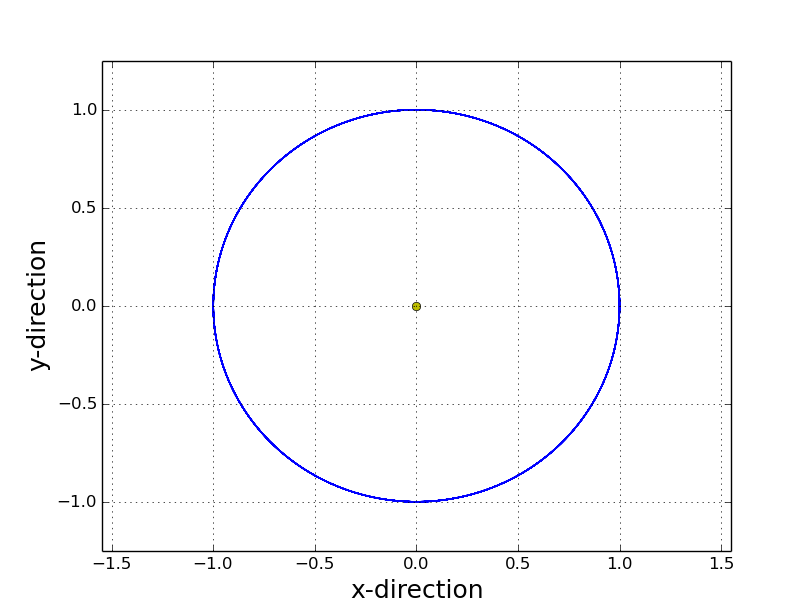
\includegraphics[scale=0.6]{oppg_3c_sun_earth_verlet_dt=10(-3)}
    \caption{The Earth's orbit, shown as a blue line, around the Sun, shown as a yellow dot. The motion is solved with VelocityVerlet, and plotted with $dt = 10^{-3}$ for a 10 year time period. The unit on both axis is AU.}
    \label{fig:EarthOrbit_Verlet_det = 10(-3)}
\end{figure}

\begin{figure} [H]
    \centering
    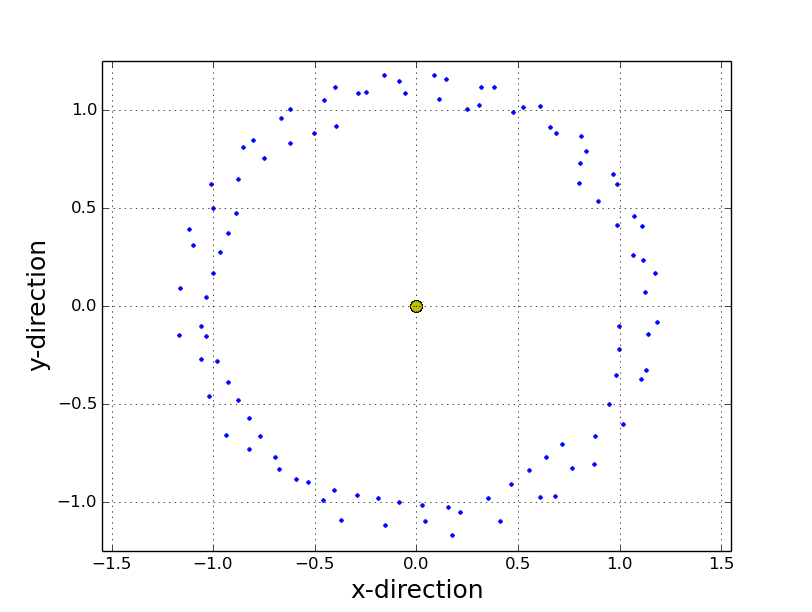
\includegraphics[scale=0.6]{oppg_3c_sun_earth_verlet_dt=10(-1)}
    \caption{The Earth's orbit, shown as blue lines, around the Sun, shown as a yellow dot. The motion is solved with VelocityVerlet, and plotted with $dt = 10^{-2}$ for a 10 year time period. The unit on both axis is AU.}
    \label{fig:EarthOrbit_Verlet_det = 10(-1)}
\end{figure}

We also compared this to the results we got when using the ODE solver EulerCromer. The plot for $dt=10^{-3}$ looked the same as Figure \ref{fig:EarthOrbit_Verlet_det = 10(-3)}. The result when using EulerCromer for $dt=10^{-1}$ is presented in Figure \ref{fig:oppg_3c_sun_earth_euler_dt=10(-1)}

\begin{figure} [H]
    \centering
    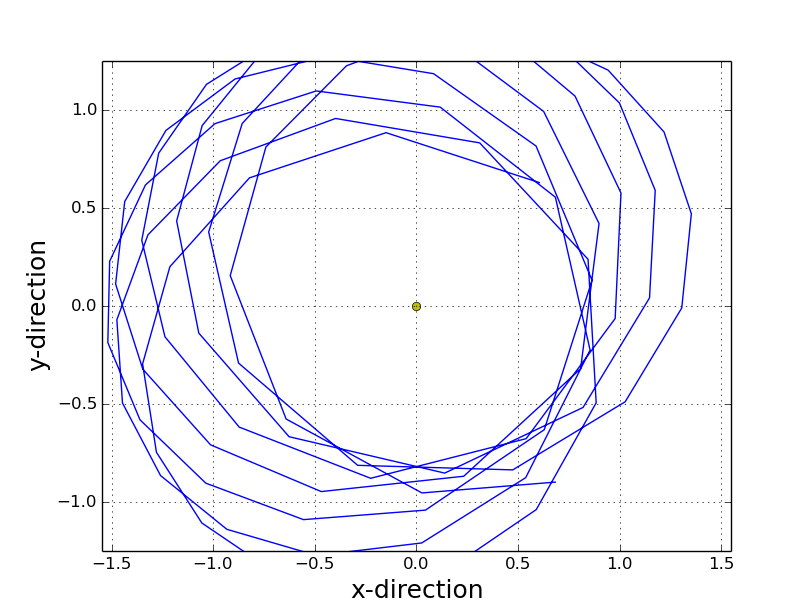
\includegraphics[scale=0.6]{oppg_3c_sun_earth_euler_dt=10(-1)}
    \caption{The Earth's orbit, shown as blue lines, around the Sun, shown as a yellow dot. The motion is solved with EulerCromer, and plotted with $dt = 10^{-1}$ for a 10 year time period. The unit on both axis is AU.}
    \label{fig:oppg_3c_sun_earth_euler_dt=10(-1)}
\end{figure}

\subsubsection{Conservation of energy and angular momentum}
We checked the conservation of total energy and angular momentum for EulerCromer and VelocityVerlet for different time steps. The results are presented in table \ref{euler_dt=10(-3)} - \ref{verlet_dt=10(-1)}
\par
\vspace{3mm}

\begin{table} [H]
\centering
\caption{Conservation of energy and angular momentum, using EulerCromer with $dt=10^{-3}$, for a 5 year period.}
\begin{tabularx}{\textwidth}{cXcXc} \toprule
    {\bf Number of Timesteps} & {\bf Total Energy }& {\bf Angular Momentum} \\
    &[$M_\odot AU^2/yr^2$]&[$M_\odot AU^2/yr$]\\ \hline
    1000 & -0.0000197 & 0.0000063\\ \hline
    2000 & -0.0000197 & 0.0000063\\ \hline
    3000 & -0.0000197 & 0.0000063\\ \hline
    4000 & -0.0000197 & 0.0000063\\ \hline
    5000 & -0.0000197 & 0.0000063\\ \bottomrule 
\end{tabularx}
\label{euler_dt=10(-3)}
\end{table}

\begin{table} [H]
\centering
\caption{Conservation of energy and angular momentum, using EulerCromer with $dt=10^{-2}$, for a 5 year period.}
\begin{tabularx}{\textwidth}{cXcXc} \toprule
    {\bf Number of Timesteps} & {\bf Total Energy }& {\bf Angular Momentum} \\
    &[$M_\odot AU^2/yr^2$]&[$M_\odot AU^2/yr$]\\ \hline
    100 & -0.0000161 & 0.0000063\\ \hline
    200 & -0.0000172 & 0.0000063\\ \hline
    300 & -0.0000183 & 0.0000063\\ \hline
    400 & -0.0000197 & 0.0000063\\ \hline
    500 & -0.0000123 & 0.0000063\\ \bottomrule 
\end{tabularx}
\label{euler_dt=10(-1)}
\end{table}

\begin{table} [H]
\centering
\caption{Conservation of energy and angular momentum, using VelocityVerlet with $dt=10^{-1}$, for a 5 year period.}
\begin{tabularx}{\textwidth}{cXcXc} \toprule
    {\bf Number of Timesteps} & {\bf Total Energy }& {\bf Angular Momentum} \\
    &[$M_\odot AU^2/yr^2$]&[$M_\odot AU^2/yr$]\\ \hline
    10 & -0.0000197 & 0.0000063\\ \hline
    20 & -0.0000196 & 0.0000063\\ \hline
    30 & -0.0000196 & 0.0000063\\ \hline
    40 & -0.0000195 & 0.0000063\\ \hline
    50 & -0.0000194 & 0.0000063\\ \bottomrule 
\end{tabularx}
\label{verlet_dt=10(-1)}
\end{table}

\subsubsection{Time, VelocityVerlet vs EulerCromer}
We ran our program with $dt = 10^{-3}$ and $100000$ grid points several times, comparing the running time of EulerCromer and VelocityVerlet. The result is presented in table \ref{timeTable}.

\begin{table} [H]
\centering
\caption{Running time for $dt=10^{-3}$ and $10^{5}$ grid points for EulerCromer and VelocityVerlet, given in seconds.}
\begin{tabularx}{\textwidth}{XccX} \toprule
    \bf EulerCromer [s] & \bf VelocityVerlet [s] \\ \hline
    0.096678 & 0.149523\\ \hline
    0.094968 & 0.156597\\ \hline
    0.093523 & 0.154659\\ \hline
    0.092571 & 0.143399\\ \hline
    0.095489 & 0.135062\\ \hline
    0.099472 & 0.146875\\ \hline
    0.102891 & 0.135980\\ \hline
    0.092515 & 0.146285\\ \bottomrule
\end{tabularx}
\label{timeTable}
\end{table}

Table \ref{timeTable} gives that the average running time for EulerCromer is $0.096018$ seconds, while the average running time for VelocityVerlet is $0.146048$ seconds for $10^{5}$ grid points.

\subsubsection{Escape Velocity}
In section 2.2.2 we calculated the analytical escape velocity for a planet in a distance $1 AU$ from the Sun, where we got $v_{esc} = 8.886 AU/yr$. Using VelocityVerlet, we tested which velocities gave the planet a total energy greater than 0. The results are presented in in table \ref{trappedTable}

\begin{table} [H]
\centering
\caption{Different initial velocities in the y-direction $(0,v_y,0)$, and whether the test showed the planet escaped or was trapped.}
\begin{tabularx}{\textwidth}{XcXcX} \toprule
    $v_y$ [AU/yr] & \bf Is the planet trapped or does it escape \\ \hline
    8.883 & trapped \\ \hline
    8.884 & trapped \\ \hline
    8.885 & trapped \\ \hline
    8.886 & escaped \\ \hline
    8.887 & escaped \\ \bottomrule
\end{tabularx}
\label{trappedTable}
\end{table}

\subsection{Three Body System}

\subsubsection{Stability of VerletVelocity for different masses of Jupiter}

\paragraph{\textbf{$M_J = 0.001M_{\odot}$}}

After implementing Jupiter with mass $M_J = 0.001M_{\odot}$ and using $dt = 10^{-3}$, we got the motion of the Three Body System over a course of 10 years, shown in Figure \ref{fig:Jupiter_m=10^(-3)_Earth_dt=10^(-3)} where we used VelocityVerlet.
\begin{figure} [H]
    \centering
    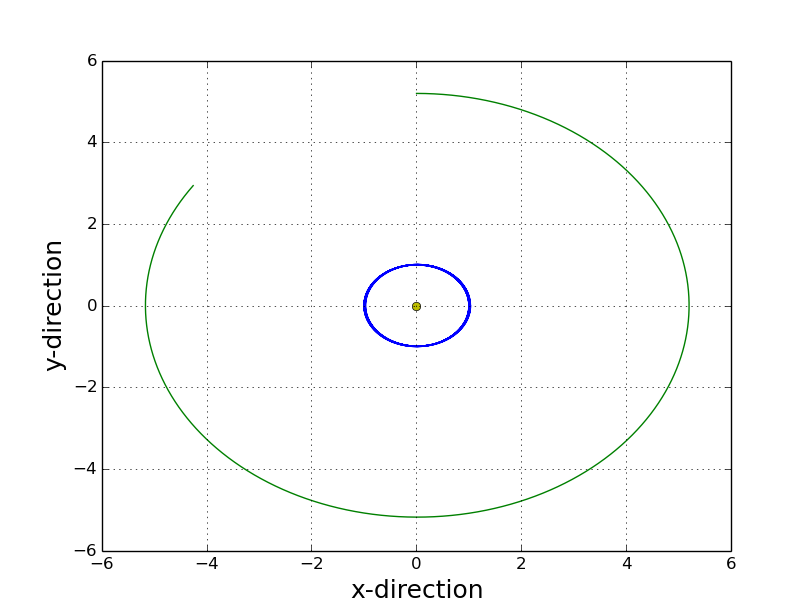
\includegraphics[scale=0.6]{oppg_3e_threebody_Jupiter_m=10_(-3)_Earth}
    \caption{The motion of the three body system, where Earth is plotted with a blue line, Jupiter with green and the Sun as a yellow dot. The plot shows the motion over a course of 10 years. We have used the time step $dt = 10^{-3}$.}
    \label{fig:Jupiter_m=10^(-3)_Earth_dt=10^(-3)}
\end{figure}

If we plot this with a larger time step, for example $dt = 10^{-1}$, we get the result as shown in Figure \ref{fig:Jupiter_m=10^(-3)_Earth_dt=10^(-1)}.

\begin{figure} [H]
    \centering
    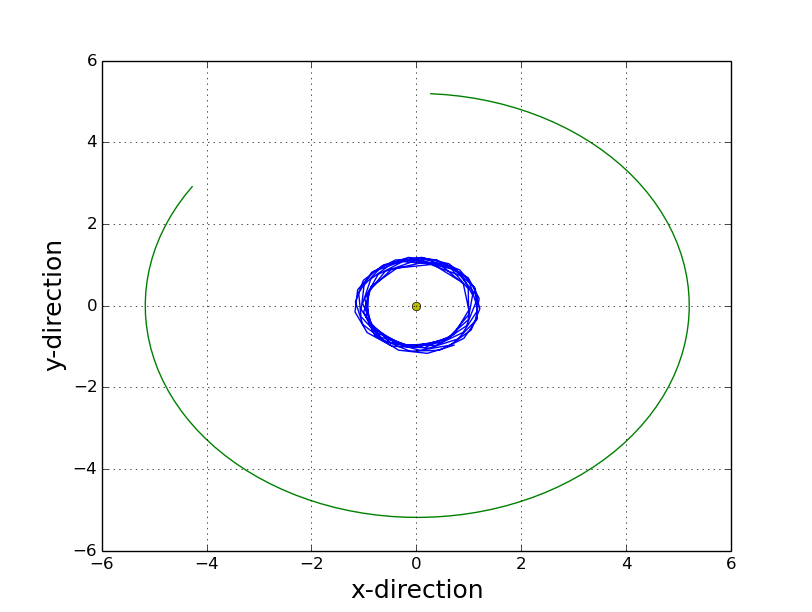
\includegraphics[scale= 0.6] {oppg_3e_threebody_Jupiter_m=10_(-3)_Earth_dt=10(-1)}
    \caption{The motion of the three body system, where Earth is plotted with a blue line, Jupiter with green and the Sun as a yellow dot. The plot shows the motion over a course of 10 years. We have used the time step $dt = 10^{-1}$.}
    \label{fig:Jupiter_m=10^(-3)_Earth_dt=10^(-1)}
\end{figure}

The conservation of energy and angular momentum  for $dt= 10^{-3}$ and $dt = 10^{-1}$ is shown in table \ref{threebody_energy_dt=10(-3)} and \ref{threebody_energy_dt=10(-1)}.

\begin{table} [H]
\centering
\caption{Conservation of energy and angular momentum for the three body system, using VelocityVerlet with $dt=10^{-3}$, over a 5 year period.}
\begin{tabularx}{\textwidth}{cXcXc} \toprule
    {\bf Number of Timesteps} & {\bf Total Energy }& {\bf Angular Momentum} \\
    &[$M_\odot AU^2/yr^2$]&[$M_\odot AU^2/yr$]\\ \hline
    1000 & -0.0038167 & 0.0143197\\ \hline
    2000 & -0.0038167 & 0.0143197\\ \hline
    3000 & -0.0038167 & 0.0143197\\ \hline
    4000 & -0.0038167 & 0.0143197\\ \hline
    5000 & -0.0038167 & 0.0143197\\ \bottomrule 
\end{tabularx}
\label{threebody_energy_dt=10(-3)}
\end{table}

\begin{table} [H]
\centering
\caption{Conservation of energy and angular momentum for the three body system, using VelocityVerlet with $dt=10^{-1}$, over a 5 year period.}
\begin{tabularx}{\textwidth}{cXcXc} \toprule
    {\bf Number of Timesteps} & {\bf Total Energy }& {\bf Angular Momentum} \\
    &[$M_\odot AU^2/yr^2$]&[$M_\odot AU^2/yr$]\\ \hline
    10 & -0.0038167 & 0.0143197\\ \hline
    20 & -0.0038166 & 0.0143197\\ \hline
    30 & -0.0038166 & 0.0143197\\ \hline
    40 & -0.0038165 & 0.0143197\\ \hline
    50 & -0.0038164 & 0.0143197\\ \bottomrule 
\end{tabularx}
\label{threebody_energy_dt=10(-1)}
\end{table}

\paragraph{\textbf{$M_J = 0.01M_{\odot}$}}

We increased the mass of Jupiter to $M_J = 0.01M_{\odot}$, and plotted the motion of the three body system. The result is shown in Figure \ref{fig:Jupiter_m=10^(-2)_Earth}.

\begin{figure} [H]
    \centering
    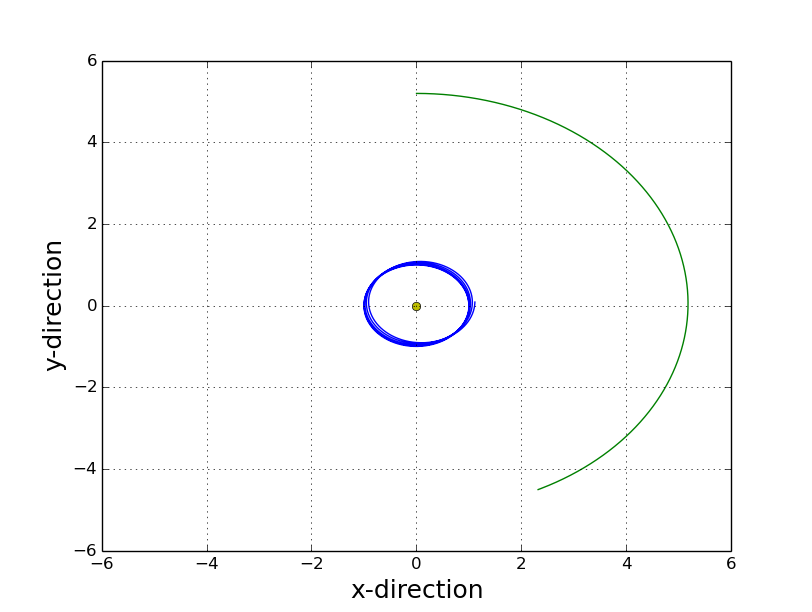
\includegraphics[scale=0.6]{oppg_3e_threebody_Jupiter_m=10_(-2)_Earth}
    \caption{The motion of the three body system, where Earth is plotted with a blue line, Jupiter with green and the Sun as a yellow dot. The mass of Jupiter is 10 times its original. The plot shows the motion over a course of 5 years. We have used the time step $dt = 10^{-3}$.}
    \label{fig:Jupiter_m=10^(-2)_Earth}
\end{figure}

\paragraph{\textbf{$M_J = M_{\odot}$}}

We increased the mass of Jupiter again, to $M_J = M_{\odot}$, and plotted the motion of the three body system. The result is shown in Figure \ref{fig:Jupiter_m=1_Earth}.

\begin{figure} [H]
    \centering
    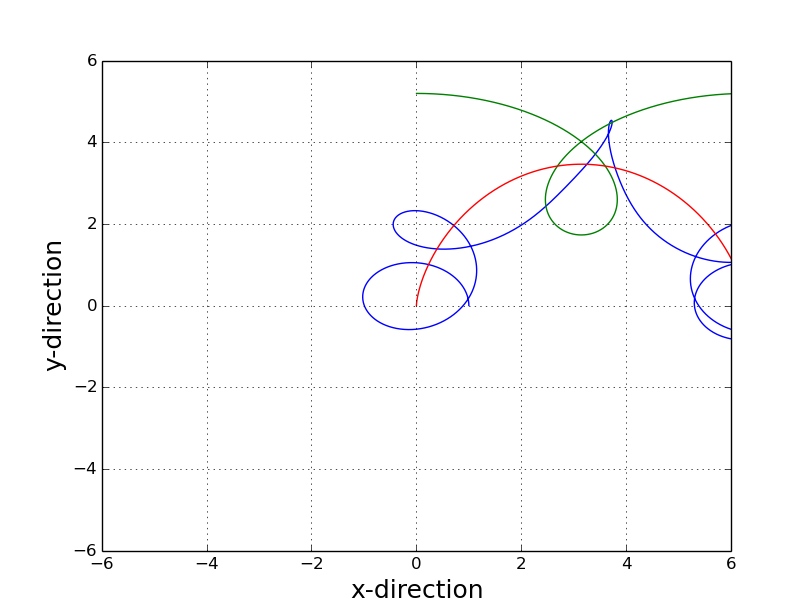
\includegraphics[scale=0.6]{oppg_3e_threebody_Jupiter_m=1_Earth}
    \caption{The motion of the three body system, where Earth is plotted with a blue line, Jupiter with green and the Sun with red. The mass of Jupiter is 1000 times its original. The plot shows the motion over the course of 5 years. We have used the time step $dt = 10^{-3}$.}
    \label{fig:Jupiter_m=1_Earth}
\end{figure}

\subsection{Solar System (many-body System)}
We implemented the eight planets of the solar system and observed that for the velocity Verlet method and time step $dt=10^{-3}$ the system was stable for at least a hundred years. 

\subsection{Mercury-Sun system}
To find the perihelion precession of Mercury, we gave Mercury initial position (0.3075, 0, 0) AU and velocity (0, 12.44, 0) AU/yr, and the sun at origo with no velocity. We also used the relativistic gravitational force (\ref{eq:GravitationalForceRelativistic}). For time step $dt=10^{-6}$ the perihelion angles, using equation \ref{eq:perihelionangle}, for ten years was found to be as shown in figure \ref{fig:precesion}. From figure \ref{fig:precesion} we get a precession of $\approx 17$ arc seconds per decade which is the same as $\approx 170$ arc seconds per century.
\begin{figure}
\centering
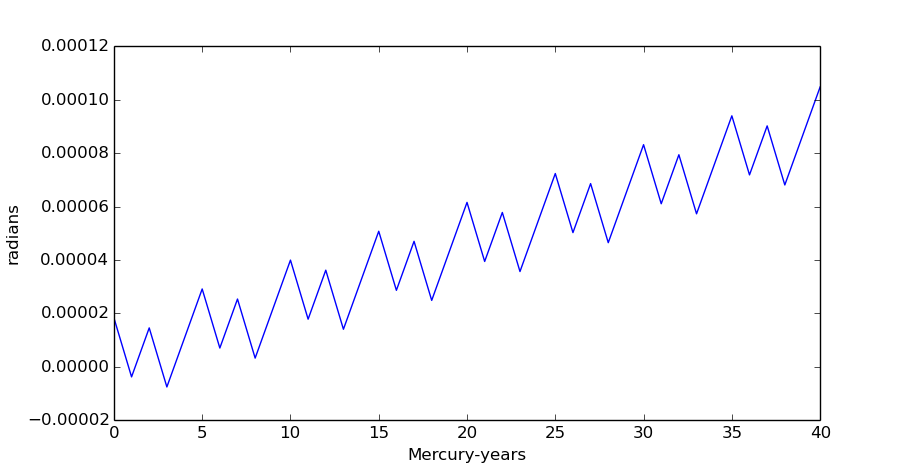
\includegraphics[scale=0.7]{precesion.png}
\caption{Plot of the perihelion angle of Mercury in radians over ten years, equivalent to forty Mercury-years. The time step used was $dt=10^{-6}$, meaning one million grid points per Earth-year.}
\label{fig:precesion}
\end{figure}

\subsection{Benchmarks}
We did some benchmarks for the two-body system to check how the numerical velocity of Earth varied for different time steps when compared to the analytical velocity calculated in Equation (\ref{eq:AnalyticVel}). The absolute error is calculated with a similar program to the one found in \textit{Test Velocity}, and the table \ref{tab:Benchmark} shows the absolute error for different times (1 $yr$, 5 $yr$, 20 $yr$ and 50 $yr$) and different time steps ($10^{-1}$ $yr$, $10^{-2}$ $yr$ and $10^{-3}$ $yr$).
\begin{table}[H]
\centering
\caption{The absolute error for the Earth-Sun system where $dt=[10^{-1}yr,10^{-2}yr,10^{-3}yr]$ calculated after 1 $yr$, 5 $yr$, 20 $yr$ and 50 $yr$.}
\label{tab:Benchmark}
\begin{tabularx}{\textwidth}{lXrXrXrXr}
\toprule
\multicolumn{5}{c}{Absolute error}\\
\midrule
$\log_{10}(dt)$ [yr]        & -1 & -2 & -3 & -4 \\
\midrule
1 $yr$      & 0.02573  & 1.34280E-08  & 2.04280E-14 & 1.18434E-07 \\
5 $yr$      & 0.34745  & 2.14846E-07  & 4.98268E-13 & 1.18445E-07 \\
20 $yr$     & 0.06115  & 5.37023E-06  & 6.50502E-12 & 1.18389E-07 \\
50 $yr$     & 0.74803  & 3.35328E-05  & 4.32525E-11 & 1.18322E-07 \\
\bottomrule
\end{tabularx}
\end{table}
The absolute error is not stable, but for $dt=10^{-2}$ and $dt=10^{-3}$ we can see a tendency - they both have increasing absolute error for longer times. For $dt=10^{-4}$ the absolute error is almost constant for all the times, and larger than for $dt=10^{-2}$ and $dt=10^{-3}$.
\section{Discussion}
In figure \ref{euler_dt=10(-1)} and \ref{fig:oppg_3c_sun_earth_euler_dt=10(-1)} we clearly see that Velocity Verlet is far superior to Euler-Cromer when it comes to numerical precision. However the Velocity Verlet was about $50\%$ more time consuming. This is also evident when looking at conservation of energy and angular momentum for $dt = 10^{-1}$, where we see that the change in energy and angular momentum is much smaller for Velocity Verlet than Euler-Cromer.

From table \ref{trappedTable} we see that our numerically calculated escape velocity for the two-body system is as we expected for time step $dt=10^{-3}$.

\par
\vspace{3mm}
When comparing the motion of the two body system in Figure \ref{fig:EarthOrbit_Verlet_det = 10(-3)} and the three body system in Figure \ref{fig:Jupiter_m=10^(-3)_Earth_dt=10^(-3)}, we observe that the Earth's orbit is slightly more elliptical after Jupiter is added. This is as expected, since the gravitational force between Earth and Jupiter drags Earth slightly out of its circular orbit. When Jupiter's mass was increased to $M_J = 0.01 M_{\odot}$, in Figure \ref{fig:Jupiter_m=10^(-2)_Earth}, we see that this drags Earth even further out of the circular orbit, and Earth spirals outwards. Finally, when $M_J = M_{\odot}$, in Figure \ref{fig:Jupiter_m=1_Earth}, the three body system becomes unstable. Theoretically we have here created a binary star system. Here we also  plot the movement of the Sun, we observe that the Sun is now visibly affected by the gravitational pull from Jupiter. Based on these plots, we conclude that our three body system behaves as we expect, and we conclude that our code works for modeling the motion of planets.\par 
By comparing Figure \ref{fig:Jupiter_m=10^(-3)_Earth_dt=10^(-3)} with Figure \ref{fig:Jupiter_m=10^(-3)_Earth_dt=10^(-1)}, we study the stability of the VerletVelocity ODE-solver for the three body system. The larger time step visibly affects the stability of the VerletVelocity solver, as it did for the two body system. 
\vspace{3mm}
\par

We saw that the Solar system is stable for 100 $yr$, but as we have seen in Equation (\ref{eq:velVerx}) and (\ref{eq:velVerv}) the integration method has errors, so we expect that the system will become unstable in the long run.
\par 
\vspace{3mm}
We found the perihelion precession of Mercury to be approximately $170$ arc seconds per century, which is more than three times what we expected. We used a time step of $dt=10^{-6}$, which in retrospect may have been to low. A reduction of the time step would have probably yielded a better result.
\par 
\vspace{3mm}

When it comes to the benchmark results, we saw that the absolute error was unstable. For $dt=10^{-1}$ the error was large as expected, and when we decreased $dt$ to $10^{-2}$, the errors were much smaller. The reason for this dramatic difference is that the error goes as $dt^3$, so it should not be surprising that the error decreases really fast for smaller time steps. The same tendency applies for $dt=10^{-3}$, but what about $dt=10^{-4}$? For $dt=10^{-4}$ the absolute error is large, something that is surprising based on the fact that we would expect an error of order $dt^3$. There can be several reasons why the error is increasing here, but the most probable is that we get truncation errors when we are finding the difference numerically. Computers with 64-bits processors is able to handle about 16 decimals, and as we can see from Table (\ref{tab:Benchmark}), the absolute error is about $10^{-14}$ when $dt=10^{-3}$. For $dt=10^{-4}$ we will have an actual absolute error of an order of $ <10^{-16}$. From the same table we can read that the error is increasing for longer times (for $dt=10^{-2}$ and $dt=10^{-3}$), something that is expected since we should have the same error for every year (every orbit). 
\section{Conclusion}
We have seen that the two- and three body systems behave as expected when given different sets of initial values, and when the whole solar system is implemented, it is stable over the course of a hundred years. This indicates that our model and implementation of the Newtonian gravitational force is correct. However for the perihelion precession of Mercury our findings where wrong, but this was probably due too insufficient time resolution. 

Furthermore, we have also seen that the ODE-solver EulerCromer is less time consuming than the VelocityVerlet solver, though VelocityVerlet is more stable and energy-conserving for larger time steps than EulerCromer.

For the benchmark we found that the error is decreasing really fast for smaller time steps when we do not deal with truncation error. For longer times the error is increasing. 
\newpage
\section{References}
\begingroup
\renewcommand{\section}[2]{}
\begin{thebibliography}{}
\bibitem{MHJ15}
  Morten Hjorth-Jensen.
  Computational Physics, Lecture Notes Fall 2015.
  Department of Physics, University of Oslo.
  August 2015.
\bibitem{Project_text}
  Project Description: 					(October 21th 2016)\newline
  \url{https://github.com/CompPhysics/ComputationalPhysics/blob/gh-pages/doc/Projects/2016/Project3/pdf/Project3.pdf}
\bibitem{NASA}
  Data from NASA: 						(October 21th 2016)\newline
  \url{http://ssd.jpl.nasa.gov/horizons.cgi}
\bibitem{kepler}
  Kepler's laws of planetary motion: 	(October 21th 2016)\newline
  \url{https://en.wikipedia.org/wiki/Kepler\%27s_laws_of_planetary_motion}
\bibitem{Barycenter}
  Barycenter: 							(October 21th 2016)\newline
  \url{http://www.uio.no/studier/emner/matnat/astro/AST1100/h14/undervisningsmateriale/lecture1.pdf}
\bibitem{solar-system-fys3150}
  Code-basis: 							(October 21th 2016)\newline
  \url{https://github.com/mortele/solar-system-fys3150}
\bibitem{Concervative_Force}
  Concervative Force:                   (October 23th 2016)\newline
  \url{https://en.wikipedia.org/wiki/Conservative_force}
\end{thebibliography}
\endgroup
\end{document}
